\documentclass[10pt, aspectratio=169]{beamer}
\usepackage{siunitx}
\usepackage[T1]{fontenc}
\usepackage{booktabs}
\usepackage[backend=biber]{biblatex}
\usepackage{mathtools,amssymb}
\usepackage{physics}
\usepackage{slashed}
\usepackage{tikz}
\usepackage{tikz-feynman}
\usepackage[list=true, font=small,
labelformat=brace, position=top]{subcaption}
% \setbeameroption{show notes on second screen} %
\addbibresource{thesis.bib}
\graphicspath{ {figs/} }

\usetheme{Antibes}
% \usepackage{eulerpx}
\usepackage{ifdraft}

% \usefonttheme[onlymath]{serif}
\setbeamertemplate{itemize items}[default]
\setbeamertemplate{enumerate items}[default]
\AtBeginSection[]
{
   \begin{frame}
       \tableofcontents[currentsection]
   \end{frame}
}

\setbeamertemplate{footline}[frame number]
\setbeamertemplate{note page}[plain]

\sisetup{separate-uncertainty = true}
% Macros

%% qqgg
\newcommand{\qqgg}[0]{q\bar{q}\rightarrow\gamma\gamma}

%% ppgg
\newcommand{\ppgg}[0]{pp\rightarrow\gamma\gamma}

%% Momenta and Polarization Vectors convenience
\DeclareMathOperator{\ps}{\slashed{p}}

\DeclareMathOperator{\pe}{\varepsilon}
\DeclareMathOperator{\pes}{\slashed{\pe}}

\DeclareMathOperator{\pse}{\varepsilon^{*}}
\DeclareMathOperator{\pses}{\slashed{\pe}^{*}}

%% Spinor convenience
\DeclareMathOperator{\us}{u}
\DeclareMathOperator{\usb}{\bar{u}}

\DeclareMathOperator{\vs}{v}
\DeclareMathOperator*{\vsb}{\overline{v}}

%% Center of Mass energy
\DeclareMathOperator{\ecm}{E_{\text{CM}}}

%% area hyperbolicus
\DeclareMathOperator{\artanh}{artanh}
\DeclareMathOperator{\arcosh}{arcosh}

%% Fast Slash
\let\sl\slashed

%% Notes on Equations
\newcommand{\shorteqnote}[1]{ &  & \text{\small\llap{#1}}}

%% Typewriter Macros
\newcommand{\sherpa}{\texttt{Sherpa}}
\newcommand{\rivet}{\texttt{Rivet}}
\newcommand{\vegas}{\texttt{VEGAS}}
\newcommand{\lhapdf}{\texttt{LHAPDF6}}
\newcommand{\scipy}{\texttt{scipy}}

%% Sherpa Versions
\newcommand{\oldsherpa}{\texttt{2.2.10}}
\newcommand{\newsherpa}{\texttt{3.0.0} (unreleased)}

%% Special Names
\newcommand{\lhc}{\emph{LHC}}

%% Expected Value and Variance
\newcommand{\EX}[1]{\operatorname{E}\qty[#1]}
\newcommand{\VAR}[1]{\operatorname{VAR}\qty[#1]}

%% Uppercase Rho
\newcommand{\Rho}{P}

%% Transverse Momentum
\newcommand{\pt}[0]{p_\mathrm{T}}

%% Sign Function
\DeclareMathOperator{\sign}{sgn}

%% Stages
\newcommand{\stone}{\texttt{LO}}
\newcommand{\sttwo}{\texttt{LO+PS}}
\newcommand{\stthree}{\texttt{LO+PS+pT}}
\newcommand{\stfour}{\texttt{LO+PS+pT+Hadr.}}
\newcommand{\stfive}{\texttt{LO+PS+pT+Hadr.+MI}}

%% GeV
\newcommand{\gev}[1]{\SI{#1}{\giga\electronvolt}}

%% Including plots
\newcommand{\plot}[2][,]{%
  \includegraphics[draft=false,#1]{./figs/#2.pdf}}
\newcommand{\rivethist}[2][,]{%
  \includegraphics[draft=false,width=\textwidth,#1]{./figs/rivet/#2.pdf}}

%% Including Results
\newcommand{\result}[1]{\input{./results/#1}\!}

\title{A Study of Monte Carlo Methods and their Application to
  Diphoton Production at the Large Hadron Collider}
\subtitle{Bachelorvortrag}
\author{Valentin Boettcher}
\beamertemplatenavigationsymbolsempty

\begin{document}
\hypersetup{pageanchor=false}
\maketitle

\hypersetup{pageanchor=true}
\pagenumbering{arabic}

\begin{frame}
  \tableofcontents
\end{frame}

\section{Introduction}
\begin{frame}{Motivation}
  \begin{block}{Monte Carlo Methods}
    \begin{itemize}
    \item (most) important numerical tools (not just) in particle
      physics
    \item crucial interface of theory and experiment
    \item enable precision predictions within and beyond SM
    \end{itemize}
  \end{block}
  \pause
  \begin{block}{Diphoton Process \(\qqgg\)}
    \begin{itemize}
    \item simple QED process, calculable by hand
    \item higgs decay channel: \(H\rightarrow \gamma\gamma\)
      \begin{itemize}
      \item instrumental in its
        discovery~\cite{Aad:2012tfa,Chatrchyan:2012ufa}
      \end{itemize}
    \item dihiggs decay \(HH\rightarrow b\bar{b}\gamma\gamma\)
      \begin{itemize}
      \item process of recent interest~\cite{aaboud2018:sf}
      \end{itemize}
    \end{itemize}
  \end{block}
\end{frame}

\section{Calculation of the \(\qqgg\) Cross Section}
\subsection{Approach}
\begin{frame}
  \begin{columns}[T]
    \begin{column}{.5\textwidth}
      \begin{figure}[ht]
        \centering
        \begin{subfigure}[c]{.28\textwidth}
          \centering
          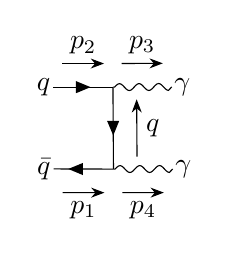
\begin{tikzpicture}[scale=.6]
            \begin{feynman}
              \diagram [small,horizontal=i2 to a] { i2
                [particle=\(q\)] -- [fermion, momentum=\(p_2\)] a --
                [fermion, reversed momentum=\(q\)] b, i1
                [particle=\(\bar{q}\)] -- [anti fermion,
                momentum'=\(p_1\)] b, i2 -- [opacity=0] i1, a --
                [photon, momentum=\(p_3\)] f1 [particle=\(\gamma\)], b
                -- [photon, momentum'=\(p_4\)] f2
                [particle=\(\gamma\)], f1 -- [opacity=0] f2, };
            \end{feynman}
          \end{tikzpicture}
          \subcaption{u channel}
        \end{subfigure}
        \begin{subfigure}[c]{.28\textwidth}
          \centering
          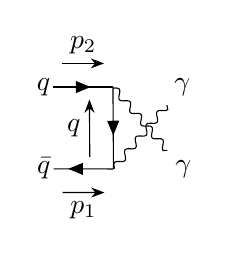
\begin{tikzpicture}[scale=.6]
            \begin{feynman}
              \diagram [small,horizontal=i2 to a] { i2
                [particle=\(q\)] -- [fermion, momentum=\(p_2\)] a --
                [fermion, reversed momentum'=\(q\)] b, i1
                [particle=\(\bar{q}\)] -- [anti fermion,
                momentum'=\(p_1\)] b, i2 -- [opacity=0] i1, a --
                [draw=none] f2 [particle=\(\gamma\)], b -- [draw=none]
                f1 [particle=\(\gamma\)], f1 -- [opacity=0] f2, };
              \diagram* { (a) -- [photon] (f1), (b) -- [photon] (f2),
              };
            \end{feynman}
          \end{tikzpicture}
          \subcaption{\label{fig:qqggfeyn2}t channel}
        \end{subfigure}
%
        \caption{Leading order diagrams for \(\qqgg\).}%
        \label{fig:qqggfeyn}
      \end{figure}
    \end{column}
    \pause
    \begin{column}{.5\textwidth}
      \begin{block}{Task: calculate
          \(\abs{\mathcal{M}}^2\)}
        \begin{enumerate}[<+->]
        \item translate diagrams to matrix elements
        \item use Casimir's trick to average over spins
        \item use completeness relation to sum over photon
          polarizations
        \item use trace identities to compute the absolute square
        \item simplify with trigonometric identities
        \end{enumerate}
      \end{block}
      \pause Here: Quark masses
      neglected.
    \end{column}
  \end{columns}
\end{frame}

\subsection{Result}

\begin{frame}
  \begin{equation}
    \label{eq:averagedm_final}
    \langle\abs{\mathcal{M}}^2\rangle = \frac{4}{3}(gZ)^4
    \cdot\frac{1+\cos^2(\theta)}{\sin^2(\theta)} =
    \frac{4}{3}(gZ)^4\cdot(2\cosh(\eta) - 1)
  \end{equation}
  %
  \pause
  \[\overset{\text{Golden Rule}}{\implies}\]
  \pause
  \begin{equation}
    \label{eq:crossec}
    \dv{\sigma}{\Omega} =
    \frac{1}{2}\frac{1}{(8\pi)^2}\cdot\frac{\abs{\mathcal{M}}^2}{\ecm^2}\cdot\frac{\abs{p_f}}{\abs{p_i}}
    = \underbrace{\frac{\alpha^2Z^4}{6\ecm^2}}_{\mathfrak{C}}\frac{1+\cos^2(\theta)}{\sin^2(\theta)}
  \end{equation}

  \pause
  \begin{figure}[ht]
    \centering
    \begin{minipage}[c]{0.3\textwidth}
      \plot[scale=.6]{xs/diff_xs}
    \end{minipage}
    \begin{minipage}[c]{0.3\textwidth}
      \caption{The differential cross section as a function of the
        polar angle \(\theta\).}
    \end{minipage}
  \end{figure}
\end{frame}

\begin{frame}{Comparison with \sherpa}
  \begin{itemize}
  \item<1-> choose \result{xs/python/eta} and \result{xs/python/ecm} and
    integrate XS
    \begin{equation}
      \label{eq:total-crossec}
      \sigma = {\frac{\pi\alpha^2Z^4}{3\ecm^2}}\cdot\qty[\tanh(\eta_2) - \tanh(\eta_1) + 2(\eta_1
      - \eta_2)]
    \end{equation}
  \item<2-> analytical result: \result{xs/python/xs}
  \item<3-> compatible with \sherpa: \result{xs/python/xs_sherpa}
  \end{itemize}
  \begin{figure}[ht]
    \centering
    \begin{minipage}[c]{0.3\textwidth}
      \plot[scale=.5]{xs/total_xs}
    \end{minipage}
    \begin{minipage}[c]{0.3\textwidth}
      \caption{\label{fig:totxs} The cross section
        of the process for a pseudo-rapidity
        integrated over \([-\eta, \eta]\).}
    \end{minipage}
  \end{figure}
\end{frame}

\section{Monte Carlo Methods}

\note[itemize]{
\item Gradually bring in knowledge through distribution.
}
\begin{frame}
  \begin{block}{Basic Ideas}
    \begin{itemize}
    \item<+-> Given some unknown function
      \(f\colon \vb{x}\in\Omega\subset\mathbb{R}^n\mapsto\mathbb{R}\) \ldots
    \item<+-> \ldots\ how do we answer questions about \(f\)?
    \end{itemize}
    \;\;\onslide<+->{\(\implies\) Sample it at random points.}
  \end{block}
  \pause
  \begin{block}{Main Applications}
    \begin{enumerate}
    \item<+-> integrate \(f\) over some volume \(\Omega\)
    \item<+-> treat \(f\) as distribution and take random samples
    \end{enumerate}
  \end{block}
\end{frame}

\subsection{Integration}
\note[itemize]{
\item omitting details (law of big numbers, central limit theorem)
\item at least three angles of attack
\item some sort of importance sampling, volume: stratified sampling
}
\begin{frame}
  \begin{itemize}
  \item<+-> we have:
    \(f\colon \vb{x}\in\Omega\subset\mathbb{R}^n\mapsto\mathbb{R}\)
    and \(\rho\colon \vb{x}\in\Omega\mapsto\mathbb{R}_{> 0}\) with
    \(\int_{\Omega}\rho(\vb{x})\dd{\vb{x}} = 1\).
  \item<+-> we seek:
    \begin{equation}
      \label{eq:baseintegral}
      I = \int_\Omega f(\vb{x}) \dd{\vb{x}}
      \onslide<+->{= \int_\Omega
        \qty[\frac{f(\vb{x})}{\rho(\vb{x})}] \rho(\vb{x}) \dd{\vb{x}} = \EX{\frac{F}{\Rho}}}
    \end{equation}
  \item<+-> numeric approximation:
    \begin{equation}
      \label{eq:approxexp}
      \EX{\frac{F}{\Rho}} \approx
      \frac{1}{N}\sum_{i=1}^N\frac{f(\vb{x_i})}{\rho(\vb{x_i})}
      \xrightarrow{N\rightarrow\infty} I
    \end{equation}
  \item<+-> error approximation:
    \begin{align}
      \sigma_I^2 &= \frac{\textcolor<+->{red}{\sigma^2}}{\textcolor<.->{blue}{N}} \\
      \sigma^2 &= \VAR{\frac{F}{\Rho}} = \int_{\textcolor<+(3)->{blue}{\Omega}} \qty[I -
      \frac{f(\vb{x})}{\textcolor<+->{blue}{\rho(\vb{x})}}]^2
      \textcolor<.->{blue}{\rho(\vb{x})} \textcolor<+->{blue}{\dd{\vb{x}}} \approx \frac{1}{N - 1}\sum_i \qty[I -
      \frac{f(\vb{x_i})}{\rho(\vb{x_i})}]^2  \label{eq:varI-approx}
    \end{align}
  \end{itemize}
\end{frame}

\begin{frame}{Change of Variables}
  Choose \(\rho(\vb{x}) = \frac{1}{\abs{\Omega}}\)
  \onslide<2->{\(\implies I=\frac{\abs{\Omega}}{N}\sum_{i=1}^N
    f(\vb{x_i})=\abs{\Omega}\cdot\bar{f}\) and
    \(\VAR{\frac{F}{P}}\approx\frac{\abs{\Omega}^2}{N-1}\sum_{i}\qty[f(\vb{x}_i)
    - \bar{f}]^2\)}
  \begin{block}{Results}
    \begin{itemize}
    \item<3-> integrating \(\dv{\sigma}{\theta}\) with target error of
      \(\sigma = \SI{1e-3}{\pico\barn}\) takes
      \result{xs/python/xs_mc_N} samples
    \item<4-> integrating \(\dv{\sigma}{\eta}\) takes just
      \result{xs/python/xs_mc_eta_N} samples
    \end{itemize}
  \end{block}
  \begin{figure}[hb]
    \centering \onslide<3->{
      \begin{subfigure}[c]{.4\textwidth}
        \centering \plot[scale=.6]{xs/xs_integrand}
      \end{subfigure}
    } \onslide<4->{
      \begin{subfigure}[c]{.4\textwidth}
        \centering \plot[scale=.6]{xs/xs_integrand_eta}
      \end{subfigure}
    }
  \end{figure}
\end{frame}

\begin{frame}{Vegas}
  \begin{columns}
    \begin{column}{.5\textwidth}
      \begin{block}{Idea}
        \begin{enumerate}
        \item subdivide integration volume into grid, take equal
          number of samples in each hypercube \(\iff\) define \(\rho\)
          as step function
        \item iteratively approximate optimal \(\rho = f(\vb{x})/I\)
          with step function
        \end{enumerate}
      \end{block}
      \begin{block}{Result}
        Total function evaluations: \result{xs/python/xs_mc_θ_vegas_N}
      \end{block}
    \end{column}
    \begin{column}{.5\textwidth}
      \begin{figure}[ht]
        \centering \plot[scale=.6]{xs/xs_integrand_vegas}
        \caption{\(2\pi\dv{\sigma}{\theta}\) scaled to increments
          found by \vegas}
      \end{figure}
    \end{column}
  \end{columns}
\end{frame}
\end{document}
